\documentclass[aspectratio=169,10pt]{beamer}
\usepackage[T1]{fontenc}
\usepackage{lmodern}
\usepackage{tikz}
\usepackage{booktabs}
\usepackage{microtype}
\usetikzlibrary{calc,positioning}

\definecolor{awesomeink}{HTML}{17191C}
\definecolor{awesomeaccent}{HTML}{E85D3F}
\definecolor{awesomemist}{HTML}{EEF0F2}
\definecolor{awesomegray}{HTML}{687078}
\setbeamercolor{normal text}{fg=awesomeink,bg=white}
\setbeamercolor{structure}{fg=awesomeaccent}
\setbeamercolor{frametitle}{fg=awesomeink,bg=white}
\setbeamercolor{title}{fg=awesomeink}
\setbeamercolor{block title}{fg=white,bg=awesomeink}
\setbeamercolor{block body}{fg=awesomeink,bg=awesomemist}
\setbeamerfont{title}{series=\bfseries,size=\LARGE}
\setbeamerfont{frametitle}{series=\bfseries,size=\Large}
\setbeamertemplate{navigation symbols}{}
\setbeamertemplate{headline}{}
\setbeamertemplate{footline}{\hbox{\begin{beamercolorbox}[wd=.16\paperwidth,ht=2.6ex,dp=1.1ex,leftskip=.35cm]{structure}\tiny\insertshortauthor\end{beamercolorbox}\begin{beamercolorbox}[wd=.60\paperwidth,ht=2.6ex,dp=1.1ex,leftskip=.2cm]{normal text}\tiny\insertshorttitle\end{beamercolorbox}\begin{beamercolorbox}[wd=.24\paperwidth,ht=2.6ex,dp=1.1ex,rightskip=.35cm plus1fil]{structure}\hfill\tiny\insertframenumber~/~\inserttotalframenumber\end{beamercolorbox}}}
\setbeamertemplate{frametitle}{\vskip.25cm\hskip.35cm\insertframetitle\hfill\color{awesomeaccent}\insertsectionnumber\hskip.35cm\par\vskip.08cm\hskip.35cm\color{awesomeaccent}\rule{\dimexpr\paperwidth-.7cm\relax}{1.2pt}}
\AtBeginSection[]{\begin{frame}[plain,noframenumbering]\begin{tikzpicture}[remember picture,overlay]\fill[awesomeink] (current page.south west) rectangle (current page.north east);\fill[awesomeaccent] (current page.south east) -- (current page.north east) -- ++(-4cm,0) -- cycle;\end{tikzpicture}\vfill\color{white}\usebeamerfont{title}\insertsectionnumber.\ \insertsection\vfill\end{frame}}

\title[Designing for the handoff]{Designing for the handoff}
\subtitle{An opinionated presentation starter}
\author[Your Name]{Your Name}
\institute{Your Team}
\date{\today}
\begin{document}
\begin{frame}[plain]
  \begin{tikzpicture}[remember picture,overlay]
    \fill[awesomeink] (current page.south west) rectangle (current page.north east);
    \fill[awesomeaccent] (current page.south east) -- (current page.north east) -- (current page.north west) -- cycle;
    \draw[white,line width=1pt] ([xshift=.8cm,yshift=.8cm]current page.south west) -- ([xshift=5.6cm,yshift=.8cm]current page.south west);
  \end{tikzpicture}
  \vfill\hspace{.6cm}\begin{minipage}{.68\paperwidth}\color{white}\usebeamerfont{title}\inserttitle\par\vspace{.2cm}\Large\insertsubtitle\par\vspace{.6cm}\normalsize\insertauthor\quad · \quad\insertinstitute\quad · \quad\insertdate\end{minipage}\vfill
\end{frame}
\begin{frame}{A short agenda}
  \tableofcontents
\end{frame}
\section{Frame the problem}
\begin{frame}{Start with the handoff}
  \begin{block}{Working thesis}
    Most friction is not inside a task; it is where one person decides that the next person has enough context.
  \end{block}
  \vspace{.4cm}
  \begin{columns}[T,onlytextwidth]
    \column{.48\textwidth}\textbf{Before}\begin{itemize}\item context lives in chat\item ownership is implied\item questions arrive late\end{itemize}
    \column{.48\textwidth}\textbf{After}\begin{itemize}\item context travels with the work\item the next owner is named\item uncertainty is visible\end{itemize}
  \end{columns}
\end{frame}
\section{Make it visible}
\begin{frame}{One screen, three signals}
  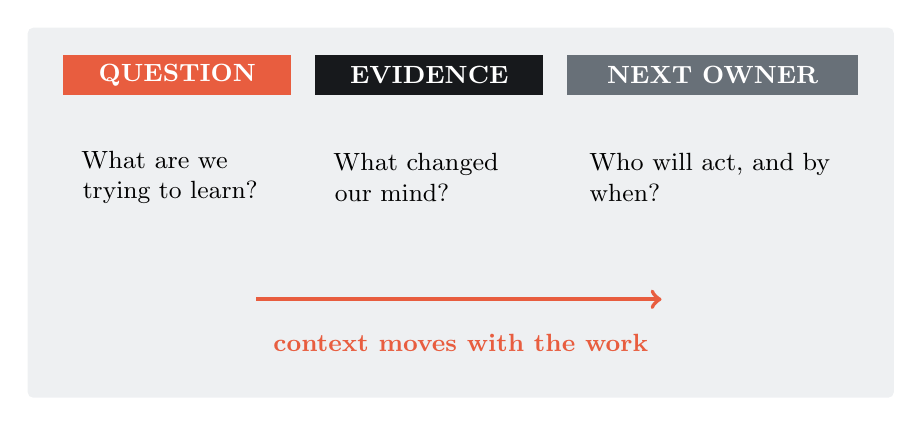
\begin{tikzpicture}[x=1cm,y=1cm]
    \fill[awesomemist,rounded corners=2pt] (0,0) rectangle (11,4.7);
    \fill[awesomeaccent] (.45,3.85) rectangle (3.35,4.35);
    \fill[awesomeink] (3.65,3.85) rectangle (6.55,4.35);
    \fill[awesomegray] (6.85,3.85) rectangle (10.55,4.35);
    \node[white,font=\small\bfseries] at (1.9,4.1) {QUESTION};
    \node[white,font=\small\bfseries] at (5.1,4.1) {EVIDENCE};
    \node[white,font=\small\bfseries] at (8.7,4.1) {NEXT OWNER};
    \node[align=left,text width=2.4cm,font=\small] at (1.9,2.8) {What are we trying to learn?};
    \node[align=left,text width=2.4cm,font=\small] at (5.1,2.8) {What changed our mind?};
    \node[align=left,text width=3.1cm,font=\small] at (8.7,2.8) {Who will act, and by when?};
    \draw[awesomeaccent,line width=1.5pt,->] (2.9,1.25) -- (8.05,1.25);
    \node[awesomeaccent,font=\small\bfseries] at (5.5,.7) {context moves with the work};
  \end{tikzpicture}
\end{frame}
\section{Close the loop}
\begin{frame}{End with a decision}
  \begin{enumerate}
    \item State the decision in one sentence.
    \item Name the next owner and checkpoint.
    \item Keep one question open for the next iteration.
  \end{enumerate}
  \vfill\centering\color{awesomeaccent}\Large\bfseries Make the handoff boring.\par\smallskip\color{awesomegray}\normalsize That is how the useful work keeps moving.
\end{frame}
\end{document}
